\documentclass[twoside]{report}

% packages
\usepackage{graphicx}
\usepackage{titlesec}
\usepackage{tocloft}
\usepackage[absolute,overlay]{textpos}
\usepackage[utf8]{inputenc}
\usepackage{fontspec}
\usepackage{setspace}
\usepackage{fancyhdr}
\usepackage{lipsum}
\usepackage{chngcntr}
\usepackage{caption}
\usepackage{booktabs} 
\usepackage{geometry}
 \geometry{
 a4paper,
 outer=22mm,
 inner=43mm,
 top=36mm,
 bottom=30mm,
 }






% configurations
\renewcommand*\contentsname{Contents}
\renewcommand{\cftchapleader}{\cftdotfill{\cftdotsep}} 
\setlength{\cftbeforechapskip}{0pt}


\newcommand\newEmptyPage{

    \newpage
    \thispagestyle{empty}
    ~\vfill
    \raggedright
    \setmainfont{GeorgiaPro-Italic}
    \fontsize{12}{14}\selectfont
    This page intentionally left blank.
    \vspace{0.5\textheight}
    \setmainfont{GeorgiaPro-Regular}

}

\defaultfontfeatures[Figtree-Medium]{
  Path = Fonts/,
  Extension = .ttf,
  }
\defaultfontfeatures[Figtree-SemiBold]{
  Path = Fonts/,
  Extension = .ttf,
  }
\defaultfontfeatures[Figtree-Regular]{
  Path = Fonts/,
  Extension = .ttf,
  }
\defaultfontfeatures[Figtree-SemiBoldItalic]{
  Path = Fonts/,
  Extension = .ttf,
  }
\defaultfontfeatures[Figtree]{
  Path = Fonts/,
  Extension = .ttf,
  UprightFont = *-Regular,
  BoldFont = *-SemiBold
  }
\newfontface\pageNumFont{Figtree-Regular}[
  Path = Fonts/,
  Extension = .ttf,
  ]

\defaultfontfeatures[GeorgiaPro-Black.ttf]{
  Path = Fonts/,
  Extension = .ttf,
  }
\defaultfontfeatures[GeorgiaPro-BlackItalic.ttf]{
  Path = Fonts/,
  Extension = .ttf,
  }
\defaultfontfeatures[GeorgiaPro-Bold.ttf]{
  Path = Fonts/,
  Extension = .ttf,
  }
\defaultfontfeatures[GeorgiaPro-BoldItalic.ttf]{
  Path = Fonts/,
  Extension = .ttf,
  }
\defaultfontfeatures[GeorgiaPro-Italic.ttf]{
  Path = Fonts/,
  Extension = .ttf,
  }
\defaultfontfeatures[GeorgiaPro-Light.ttf]{
  Path = Fonts/,
  Extension = .ttf,
  }
\defaultfontfeatures[GeorgiaPro-LightItalic.ttf]{
  Path = Fonts/,
  Extension = .ttf,
  }
\defaultfontfeatures[GeorgiaPro-Regular.ttf]{
  Path = Fonts/,
  Extension = .ttf,
  }
\defaultfontfeatures[GeorgiaPro-SemiBold.ttf]{
  Path = Fonts/,
  Extension = .ttf,
  }
\defaultfontfeatures[GeorgiaPro-SemiBoldItalic.ttf]{
  Path = Fonts/,
  Extension = .ttf,
  }


\titleformat{\chapter}[hang]{\normalfont\fontsize{24}{28}\selectfont\bfseries\fontspec{Figtree-Medium}}{\hspace*{-1cm}\thechapter}{20pt}{}
\titlespacing{name=\chapter}{-0.2cm}{17pt}{18pt}

\setcounter{secnumdepth}{3}

\titleformat{\section}[hang]{\normalfont\fontsize{13}{15}\selectfont\bfseries\fontspec{Figtree-SemiBold}\raggedright}{\thesection}{1ex}{}
\titlespacing{\section}{0cm}{12pt}{12pt}

\titleformat{\subsection}[hang]{\normalfont\fontsize{12}{14}\selectfont\bfseries\fontspec{Figtree-SemiBold}\raggedright}{\thesubsection}{1ex}{}
\titlespacing{\subsection}{0cm}{12pt}{10pt}

\titleformat{\subsubsection}[hang]{\normalfont\fontsize{12}{14}\selectfont\bfseries\fontspec{Figtree-SemiBoldItalic}\raggedright}{\thesubsubsection}{1ex}{}
\titlespacing{\subsubsection}{0cm}{12pt}{10pt}


\counterwithout{figure}{chapter}
\counterwithout{table}{chapter}


\fancypagestyle{plain}{
    \fancyhf{} 
    \fancyfoot[RO]{\pageNumFont\fontsize{9}{10}\selectfont\thepage} % Right side on odd pages
    \fancyfoot[LE]{\pageNumFont\fontsize{9}{10}\selectfont\thepage} % Left side on even pages
    \setlength{\footskip}{2cm}
    \setlength{\marginparwidth}{2cm}
    \renewcommand{\headrulewidth}{0pt} 
    \renewcommand{\footrulewidth}{0pt}
}

\fancypagestyle{empty}{
    \fancyhf{}
    \renewcommand{\headrulewidth}{0pt} 
    \renewcommand{\footrulewidth}{0pt}
}




\begin{document}



\newcommand\SubjectArea{Degree Project in Optimization and Systems Theory}

\newcommand\Cycle{Second cycle, 30 credits}

\newcommand\ThesisTitle{Clustering Financial Profiles: Evaluating Segmentation Effectiveness on Customer Bank Data}

\newcommand\ThesisSubtitle{A Comprehensive Study on Unsupervised Clustering Methods for High-Dimensional Financial Profile Data}


\newcommand\ThesisAuthor{Anh Do}

\newcommand\TitlePageText{
    Master’s Programme, Applied and Computational Mathermatic, Optimization and Systems Theory track\break
    Supervisor: \break
    Examiner: \break
    School of Engineering Sciences\break
    Host company: TF Bank AB\break
    Swedish title: Klustering av finansiella profiler: Utvärdering av segmenteringens effektivitet för finansiella kunddata\break
    Swedish subtitle: En omfattande studie av oövervakade klusteringsmetoder för högdimensionell finansiell kunddata
    
}
\newcommand\AddCompanyLogo{
    
\includegraphics[width=2cm]{Figures/Avarda_bank_logo_2024.svg.png}
} %leave empty if no company 


\newcommand\AbstractEnglish{
The application of modern mathematical methods within financial institutions is well established, particularly in areas such as asset pricing, credit risk assessment, and portfolio optimization, where advanced mathematical modeling forms the core analytical foundation. In contrast, more traditional tasks such as customer segmentation have historically relied on manual rule-based approaches and domain-specific business knowledge rather than formal mathematical frameworks.

This thesis investigates the feasibility and effectiveness of applying unsupervised clustering methods to customer segmentation using high-dimensional financial data. The study presents a complete methodological pipeline, beginning with raw transactional and account-level data and proceeding through feature construction, normalization, dimensional control, and distance-based clustering. Emphasis is placed on the mathematical challenges inherent to clustering in high-dimensional spaces, including metric selection, feature scaling, correlation, and robustness to skewed distributions.

Using distance-based unsupervised learning algorithms, the resulting clusters are evaluated through internal validation measures and statistical comparison of cluster-specific feature distributions. The thesis further examines the temporal stability of cluster assignments across consecutive periods. The results demonstrate both the potential and the limitations of unsupervised clustering as a mathematically grounded approach to customer segmentation in financial data.
}

\newcommand\KeywordsEnglish{
Unsupervised clustering,
High-dimensional data,
Distance metrics,
Feature preprocessing,
Applied mathematics
}

\newcommand\AbstractSwedish{
Användningen av moderna matematiska metoder inom finansiella institutioner är sedan länge väletablerad, särskilt inom områden som tillgångsprissättning, kreditriskbedömning och portföljoptimering, där avancerad matematisk modellering utgör den centrala analytiska grunden. Däremot har mer traditionella uppgifter, såsom kundsegmentering, historiskt sett i större utsträckning baserats på manuella regelbaserade metoder och domänspecifik affärskunskap snarare än formella matematiska ramverk.

Denna examensarbete undersöker möjligheterna och effektiviteten hos oövervakade klusteringsmetoder för kundsegmentering baserad på högdimensionell finansiell data. Studien presenterar en komplett metodologisk pipeline, från rå transaktions- och kontodata till konstruktion av egenskaper, normalisering, dimensionskontroll och avståndsbaserad klustering. Särskild tonvikt läggs vid de matematiska utmaningar som är förknippade med klustering i högdimensionella rum, inklusive val av metriker, egenskapsskalning, korrelation samt robusthet mot snedfördelade variabler.

Med hjälp av avståndsbaserade oövervakade inlärningsalgoritmer utvärderas de resulterande klustren genom interna valideringsmått samt statistiska jämförelser av klusterspecifika egenskapsfördelningar. Vidare analyseras den temporala stabiliteten hos klustertillhörighet över på varandra följande tidsperioder. Resultaten påvisar både potentialen och begränsningarna hos oövervakad klustering som en matematiskt förankrad metod för kundsegmentering av finansiell data.
}

\newcommand\KeywordsSwedish{
Oövervakad inlärning,
Högdimensionell data,
Avståndsbaserade metoder,
Dataförberedelse,
Tillämpad matematik
}

\newcommand\AbbreviationsList{
\begin{description}
    \item[IQR] Interquartile Range
    \item[NZV] Near-Zero Variance
    \item[PCA] Principal Component Analysis
    \item[RFM] Recency, Frequency, Monetary
    \item[UMAP] Uniform Manifold Approximation and Projection
    \item[WCSS] Within-Cluster Sum of Squares
\end{description}
}

\newcommand\Acknowledgments{
I would like to express my sincere gratitude to Hampus Nyquist, Wilhelm Back, Yueqi Cao, and Carlos Eduardo for their support throughout the entire process, from data processing to modeling and validation.
}

  %%%%% cover page %%%%%
\pagestyle{plain}
\pagenumbering{gobble}
\begin{textblock*}{\paperwidth}(0cm,1.25cm)
    \centering 
    
\includegraphics[width=3.75cm]{Figures/KTH_logo.png}
\end{textblock*}

\begin{textblock*}{15.86cm}(2.63cm, 8.62cm)
    \setmainfont{Arial}
    \centering 
    \fontsize{12}{14}\selectfont
    \SubjectArea\
    \break
    \fontsize{10}{14}\selectfont
    \Cycle\
\end{textblock*}

\begin{textblock*}{15.86cm}(2.63cm, 11.13cm)
    \setmainfont{Arial}
    \centering        
    \begin{spacing}{1.5}
    \fontsize{24}{20}\selectfont
    \textbf{ \ThesisTitle\ }
    \end{spacing}    
    \break
    \break
    \fontsize{16}{20}\selectfont
    \ThesisSubtitle\ 
    \break
    \break
    \fontsize{12}{20}\selectfont
    \MakeUppercase{\textbf{ \ThesisAuthor\ }} 
\end{textblock*}

~\newEmptyPage\
\newpage

  %%%%% title page %%%%%

\begin{textblock*}{\paperwidth}(0cm,1.25cm) 
    \centering 
    
\includegraphics[width=3cm]{Figures/KTH_logo.png}
\end{textblock*}

\vspace*{2cm}
\setmainfont{Figtree}
\raggedleft  
    \begin{spacing}{1.2}
\fontsize{24}{26}\selectfont
     \ThesisTitle\    
     \end{spacing}
\fontsize{16}{20}\selectfont
    \ThesisSubtitle\ \break  \break

\fontsize{16}{20}\selectfont

 \ThesisAuthor\ 
 
\vfill
 \raggedright
 \setmainfont{GeorgiaPro-Regular}
 \fontsize{12}{14}\selectfont
\TitlePageText\

 \raggedleft
  \AddCompanyLogo\  

\newEmptyPage\
\setlength{\parskip}{5.25pt}
  %%%%% Abstracts %%%%%

\chapter*{Abstract}
    \raggedright
    \setmainfont{GeorgiaPro-Regular}
    \fontsize{12}{14}\selectfont
    \AbstractEnglish\
    
    \setmainfont{GeorgiaPro-Bold}
    \vspace*{1cm}
    Keywords
    
    \setmainfont{GeorgiaPro-Regular}
    \KeywordsEnglish\
    
\newEmptyPage\

\chapter*{Sammanfattning}
   \raggedright
    \setmainfont{GeorgiaPro-Regular}
    \fontsize{12}{14}\selectfont
    \AbstractSwedish\
    
    \setmainfont{GeorgiaPro-Bold}
    \vspace*{1cm}
    Keywords
    
    \setmainfont{GeorgiaPro-Regular}
    \KeywordsSwedish\


\newEmptyPage\
  %%%%% Acknowledgments and contents %%%%%
\chapter*{Acknowledgments}
\Acknowledgments\
\newEmptyPage\

\chapter*{List of Abbreviations}
\AbbreviationsList\
\newEmptyPage\

\setmainfont{Figtree-Regular}
\tableofcontents

\newEmptyPage\


\newpage
\pagenumbering{arabic}
\setcounter{page}{1}




 

% add \newEmptyPage\  before chapters name if chapters starts on even page

\chapter{Introduction}
\section{Context and Motivation}
The modern financial services industry relies heavily on data-driven decision-making to manage credit card portfolios, assess customer segments, target audiences, and optimize campaign profitability \cite{sargeant_algorithmic_2023}. However, much of this segmentation currently depends on manually defined rules and heuristics, which are typically formulated through an analyst's extensive, hands-on experience with the data.

However, this manual approach is inherently unscalable. As data volumes grow and the dimensionality of available features increases, human-driven analysis can only accommodate an ever-decreasing fraction of the true complexity within the customer base. To overcome these limitations, unsupervised machine learning offers a promising, data-driven alternative. The objective of applying this methodology is not merely to search for hidden anomalies, but first and foremost to demonstrate that algorithmic approaches can reliably identify and group standard, expected behavioral patterns. By successfully capturing this foundational business logic as a baseline, the method can then be further leveraged to uncover complex, latent customer segments derived from highly nuanced account behavior. Ultimately, this research aims to show how such techniques can provide a comprehensive and scalable segmentation strategy free from rigid, predefined assumptions.

\section{Problem Statement}
Despite the availability of comprehensive transactional and profitability data, translating these raw operational databases into cohesive customer segments presents a significant engineering and analytical challenge. Financial datasets are inherently complex: they are characterized by millions of records, high dimensionality, and multiple time horizons. Furthermore, transactional columns are frequently sparse (zero-heavy), which poses a unique hurdle for unsupervised learning algorithms to process effectively.

The core problem addressed in this thesis is the design and implementation of an end-to-end data processing and clustering pipeline capable of navigating this complexity. To generate meaningful insights, the raw data must be carefully aggregated, filtered, and engineered to ensure that highly correlated features do not skew the results. Ultimately, the challenge lies in building a scalable methodology that can distill raw financial data into distinct, economically interpretable customer segments.

\section{Research Objectives}
To address this problem, this thesis is guided by the following primary research objectives:

\begin{enumerate}
    \item \textbf{Develop a Scalable Data Aggregation Pipeline:} Construct a robust methodology to merge and summarize diverse financial databases into unified annual feature profiles.
    
    \item \textbf{Execute Unsupervised Customer Segmentation:} Apply clustering algorithms to the engineered dataset to empirically identify distinct groups of credit card agreements, utilizing quantitative scoring metrics to determine the optimal number of segments.
    
    \item \textbf{Profile Financial and Behavioral Characteristics:} Interpret the resulting clusters by analyzing their defining features, such as spending behavior across different categories
\end{enumerate}

\section{Scope and Limitations}
\label{sec:limitations}
The scope of this research is defined by a targeted sample of approximately 500000 unique credit card agreements, focusing specifically on annual aggregated data for the years 2024 and 2025.

A primary limitation of this study is the inherent nature of unsupervised learning; because the data lacks ground-truth customer labels, validation relies on internal mathematical heuristics rather than predictive accuracy. Additionally, by aggregating to an annual level, seasonality and short-term behavioral shifts may be smoothed over or obscured.

\section{Thesis Structure}
The remainder of this thesis is structured as follows. Chapter \ref{chap:Background} provides the theoretical background, detailing the financial metrics and unsupervised machine learning algorithms utilized in this study. Chapter \ref{chap:Methodology} outlines the methodology, documenting the data engineering pipeline, feature selection process, and the experimental setup for the clustering model. Chapter \ref{chap:Results} presents the results, illustrating the optimal cluster formations and providing a detailed financial interpretation of each customer segment. Finally, Chapter 5 concludes the thesis by discussing the business implications of these findings and proposing avenues for future research.

\chapter{Background}
\label{chap:Background}
This chapter establishes the theoretical foundation for the methodologies applied in this research. It first explores the domain of credit card portfolio management and standard financial metrics. Subsequently, it details the mathematical principles behind unsupervised machine learning, specifically focusing on dimensionality reduction techniques, clustering algorithms, and the quantitative metrics used to evaluate them.

    \section{Customer Segmentation in Retail Banking}
    \label{sec:banking_segmentation}
    In the financial services sector, credit card portfolios represent a complex ecosystem of customer behaviors, borrowing habits, and repayment patterns. Traditionally, institutions segmented these portfolios by applying manually defined rules to frameworks like the RFM (Recency, Frequency, Monetary) model to assess risk and profitability. 
    
    In a retail banking context, this framework evaluates three core dimensions of account activity: \textit{Recency} measures the time elapsed since a customer's last transaction, indicating their current engagement level; \textit{Frequency} captures the total volume of transactions within a specific period, serving as a proxy for card reliance; and \textit{Monetary} quantifies the total transaction value or outstanding balance, directly tying customer behavior to institutional profitability \cite{wilbert_recency_2023}.
    
    While this manual, rule-based approach is effective for simple datasets, it struggles to scale and capture the nuances of high-dimensional data. Consequently, modern analytical approaches do not discard these foundational metrics; instead, they integrate core RFM variables with additional behavioral and demographic features to serve as inputs for unsupervised machine learning models. This evolution allows institutions to algorithmically discover latent, multivariate patterns rather than relying on rigid, human-defined heuristics \cite{yan_bank_2025}.

    \section{Unsupervised Machine Learning}
    \label{sec:unsupervised_ml}

    Unlike supervised machine learning, which relies on a set of labeled training data to predict a known target variable, unsupervised machine learning focuses on discovering hidden structures and intrinsic patterns within unlabeled datasets. The primary objective of an unsupervised algorithm is not to map inputs to a predefined output, but rather to infer the natural topology, relationships, or distributions inherent in the data itself \cite{naeem_unsupervised_2023}.
    
    In the context of financial customer segmentation, ground-truth labels defining distinct "customer archetypes" are rarely known in advance. While traditional approaches attempt to force customers into rigid, predefined demographic or financial buckets, unsupervised learning provides a purely data-driven methodology. By algorithmically evaluating the multivariate similarities across diverse account features, such as transaction categories, utilization rates, and repayment behaviors, unsupervised models can autonomously partition the customer base into cohesive, economically meaningful segments without human bias.
    
        \subsection{K-means}
        \label{subsec:kmeans}
        
        In our study our primary focus will be on the $K$-means clustering algorithm \cite{naeem_unsupervised_2023}. Its computational efficiency and robust theoretical foundation make it particularly well-suited for partitioning large-scale, multidimensional financial datasets.
        
        The $K$-means algorithm aims to partition a given dataset into $K$ distinct, non-overlapping clusters by minimizing the intra-cluster variance, commonly referred to as the Within-Cluster Sum of Squares (WCSS). Let our financial dataset be represented as an $n \times d$ matrix, where we have $n$ observations $X = \{x_1, x_2, \dots, x_n\}$ and each observation $x_i \in \mathbb{R}^d$ is a $d$-dimensional vector of financial features. We seek to partition the dataset into a set of $K$ clusters $S = \{S_1, S_2, \dots, S_K\}$, where $K \le n$.
        
        The formal objective is to find the assignment of data points to clusters that minimizes the following cost function:
        
        \begin{equation}
        \label{eq:kmeanscost}
            J(S) = \sum_{i=1}^{K} \sum_{x \in S_i} \|x - \mu_i\|^2
        \end{equation}
        
        where $\mu_i$ represents the geometric centroid (or mean) of the points assigned to cluster $S_i$, and $\|x - \mu_i\|^2$ denotes the squared Euclidean distance between a data point and its respective cluster centroid.
        
        Because finding the exact global optimum for this problem is NP-hard, $K$-means typically employs an iterative refinement technique known as Lloyd's algorithm. The process begins by initializing $K$ centroids, $\mu_1^{(0)}, \mu_2^{(0)}, \dots, \mu_K^{(0)}$, often chosen randomly from the dataset or via methods such as $K$-means++ to improve convergence speed and avoid poor local minima \cite{arthur_k-means_2007}. The algorithm then alternates between two core operations:
        
        \begin{enumerate}
            \item \textbf{Assignment Step:} Each data point is assigned to the cluster whose centroid yields the least squared Euclidean distance. For the $t$-th iteration, the updated cluster $S_i^{(t)}$ is defined mathematically as:
            \begin{equation}
                S_i^{(t)} = \left\{ x_p : \|x_p - \mu_i^{(t)}\|^2 \le \|x_p - \mu_j^{(t)}\|^2 \ \forall j, 1 \le j \le K \right\}
            \end{equation}
        
            \item \textbf{Update Step:} Once all data points have been assigned, the new centroids for the $(t+1)$-th iteration are recalculated as the center of mass of the points in each respective cluster:
            \begin{equation}
                \mu_i^{(t+1)} = \frac{1}{|S_i^{(t)}|} \sum_{x_j \in S_i^{(t)}} x_j
            \end{equation}
        \end{enumerate}
        
        These two steps are repeated iteratively until convergence is achieved—specifically, when the cluster assignments no longer change ($S_i^{(t)} = S_i^{(t-1)}$), or when a predefined tolerance for the reduction in WCSS is met. By mathematically minimizing the variance within each grouping, the algorithm organically isolates distinct customer archetypes defined by their shared multivariate financial behaviors.
        
        \subsection{Mini-Batch K-means}
        \label{subsec:minibatch_kmeans}
        
        The principles of stochastic descent provide the theoretical foundation for the Mini-Batch $K$-means algorithm (see Section \ref{sec:descent_optimization}). As established in Equation \ref{eq:kmeanscost}, the $K$-means cost function (WCSS) is inherently non-convex, meaning optimization relies on finding a stable local minimum.
        
        In standard $K$-means (Lloyd's algorithm), computing the distance between all $n$ points and $K$ centroids during the assignment step is analogous to a full batch evaluation, which scales poorly. Mini-Batch $K$-means mitigates this by applying stochastic optimization to the centroid updates \cite{sculley_web-scale_2010}.
        
        At iteration $t$, a random mini-batch $B$ of size $b$ is drawn from the dataset. Let $B_i \subset B$ represent the subset of points in the mini-batch assigned to the $i$-th centroid, $\mu_i$. Instead of replacing the centroid entirely, the algorithm performs an incremental update that shifts the centroid toward the mean of the new data points. This is fundamentally a stochastic gradient descent step on the WCSS cost function.
        
        Crucially, the algorithm maintains a per-center count, $v_{i, t}$, which tracks the cumulative number of data points assigned to centroid $\mu_i$ up to iteration $t$. The centroid is updated as follows:
        
        \begin{equation}
            \mu_i^{(t+1)} = \mu_i^{(t)} + \frac{1}{v_{i, t}} \sum_{x \in B_i} \left( x - \mu_i^{(t)} \right)
        \end{equation}
        
        This update mechanism elegantly reveals the underlying learning rate of the algorithm: $\alpha_t = \frac{1}{v_{i, t}}$. Because the cumulative point count $v_{i, t}$ increases linearly with the number of iterations, the learning rate decays proportionally to $1/t$. 
        
        This specific decay rate perfectly satisfies the Robbins-Monro convergence criteria (Equation \ref{eq:robbins_monro}), since the harmonic series diverges ($\sum \frac{1}{t} = \infty$) while the sum of its squares converges ($\sum \frac{1}{t^2} < \infty$). Therefore, Mini-Batch $K$-means is theoretically guaranteed to converge to a stable local optimum. By framing the centroid shifts as stochastic gradient updates with a naturally decaying learning rate, the algorithm achieves drastic reductions in computational complexity without sacrificing theoretical convergence guarantees.
    
        \subsection{K-median}
        \label{subsec:kmedian}
        
        While the $K$-means algorithm is computationally efficient, its reliance on squared Euclidean distances makes it inherently sensitive to outliers. In financial datasets, where extreme values are common, these outliers can disproportionately skew the cluster centroids. To address this vulnerability, the $K$-median clustering algorithm serves as a robust alternative.
        
        Instead of minimizing the variance, $K$-median aims to partition the dataset by minimizing the absolute deviations between data points and their cluster centers. Using the same dataset matrix $X$ and cluster set $S$ defined previously, the formal objective of $K$-median is to find the assignment that minimizes the following cost function:
        
        \begin{equation}
        \label{eq:kmediancost}
            J_{median}(S) = \sum_{i=1}^{K} \sum_{x \in S_i} \|x - m_i\|_1
        \end{equation}
        
        where $m_i$ represents the median vector of the points assigned to cluster $S_i$, and $\|x - m_i\|_1$ denotes the $L_1$ norm, commonly known as the Manhattan distance, between a data point and its cluster median. 
        
        Similar to $K$-means, the optimization of this cost function is achieved through an iterative heuristic framework. After initializing $K$ medians, $m_1^{(0)}, m_2^{(0)}, \dots, m_K^{(0)}$, the algorithm alternates between the following two operations:
        
        \begin{enumerate}
            \item \textbf{Assignment Step:} Each data point is assigned to the cluster whose median yields the smallest $L_1$ distance. For the $t$-th iteration, the assignment is mathematically defined as:
            \begin{equation}
                S_i^{(t)} = \left\{ x_p : \|x_p - m_i^{(t)}\|_1 \le \|x_p - m_j^{(t)}\|_1 \ \forall j, 1 \le j \le K \right\}
            \end{equation}
        
            \item \textbf{Update Step:} Once all data points are assigned, the new median for the $(t+1)$-th iteration is computed. Unlike the arithmetic mean, the multidimensional median is calculated independently for each feature dimension $f$:
            \begin{equation}
                (m_i^{(t+1)})_f = \text{median} \left( \{ (x_j)_f : x_j \in S_i^{(t)} \} \right) \quad \forall f \in \{1, 2, \dots, d\}
            \end{equation}
            where $(m_i)_f$ and $(x_j)_f$ denote the $f$-th feature component of the respective vectors.
        \end{enumerate}
        
        These steps repeat until convergence. By substituting the mean with the median and the squared $L_2$ norm with the $L_1$ norm, the $K$-median algorithm effectively prevents extreme financial anomalies from dominating the spatial definition of the clusters, resulting in more representative and economically stable customer archetypes.

        \subsection{Principal Component Analysis (PCA)}
        \label{subsec:pca}
        
        While partitioning algorithms like $K$-means and $K$-median group observations into distinct clusters, financial datasets are frequently characterized by high dimensionality. As the number of features $d$ increases, the concept of distance becomes inherently less discriminative, this is a mathematical phenomenon widely known as the curse of dimensionality. To mitigate this, Principal Component Analysis (PCA) is often employed as a preliminary unsupervised learning step to reduce the feature space while preserving the maximum possible variance of the original dataset \cite{naeem_unsupervised_2023}.
        
        Given our centered dataset matrix $X \in \mathbb{R}^{n \times d}$ (where the empirical mean of each feature column has been shifted to zero), PCA seeks an orthogonal linear transformation that projects the data into a new $k$-dimensional subspace, where $k < d$. The objective is to find a set of $k$ orthogonal direction vectors, known as principal components, that maximize the variance of the projected data.
        
        The spatial relationships between the features are captured by the $d \times d$ sample covariance matrix, defined mathematically as:
        \begin{equation}
            \Sigma = \frac{1}{n-1} X^T X
        \end{equation}
        
        To find the principal components that maximize variance, we solve the algebraic eigenvalue problem for the covariance matrix:
        \begin{equation}
            \Sigma w_j = \lambda_j w_j
        \end{equation}
        
        where $w_j \in \mathbb{R}^d$ represents the $j$-th eigenvector and $\lambda_j$ is its corresponding eigenvalue. In this context, the eigenvector dictates the direction of the principal axis, while the eigenvalue strictly quantifies the magnitude of the dataset's variance explained along that specific axis. 
        
        By sorting the eigenvalues in descending order ($\lambda_1 \ge \lambda_2 \ge \dots \ge \lambda_d$), we identify the orthogonal directions that capture the most intrinsic information. The first $k$ eigenvectors are concatenated to form the projection matrix $W_k = [w_1, w_2, \dots, w_k] \in \mathbb{R}^{d \times k}$. The original high-dimensional dataset is then mapped into the reduced subspace via the linear transformation:
        \begin{equation}
            X_{reduced} = X W_k
        \end{equation}
        
        In the context of financial customer segmentation, applying PCA prior to $K$-means clustering effectively filters out stochastic noise and redundant, collinear variables (such as highly correlated transaction categories). This dimensionality reduction not only accelerates the iterative descent optimization discussed in Section \ref{sec:descent_optimization}, but also stabilizes the resulting cluster assignments by grounding the Euclidean distance calculations exclusively in the most statistically significant dimensions.

        \subsection{Uniform Manifold Approximation and Projection (UMAP)}
        \label{subsec:umap}
        
        While Principal Component Analysis (PCA) (see Section \ref{subsec:pca}) provides an efficient mechanism for capturing the global variance and linear relationships within a dataset, it inherently struggles to resolve complex, non-linear patterns. In high-dimensional financial datasets, data points frequently lie on complex, non-linear manifolds that linear projections simply flatten, causing distinct behavioral groups to overlap. To address this limitation, non-linear dimensionality reduction techniques are often employed. While algorithms such as t-Distributed Stochastic Neighbor Embedding (t-SNE) have historically been popular for these tasks, this research incorporates Uniform Manifold Approximation and Projection (UMAP) \cite{mcinnes_umap_2020} as an auxiliary, exploratory tool due to its superior computational scalability and robust theoretical foundation. Consequently, t-SNE will not be covered in detail in this study.
        
        UMAP is a modern manifold learning technique grounded in Riemannian geometry and algebraic topology. Unlike PCA, which mathematically projects data onto orthogonal axes that maximize variance, UMAP operates by constructing a high-dimensional fuzzy topological representation (a weighted graph) of the data and subsequently optimizing a low-dimensional graph to be as structurally similar as possible. This optimization is achieved by minimizing the fuzzy set cross-entropy $C$ between the high-dimensional graph weights $v_{i,j}$ (representing the likelihood that two points are connected in the original space) and the low-dimensional graph weights $w_{i,j}$ (representing their connectivity in the embedded space):
        
        \begin{equation}
            C = \sum_{i \neq j} \left( v_{i,j} \log\left(\frac{v_{i,j}}{w_{i,j}}\right) + (1 - v_{i,j}) \log\left(\frac{1 - v_{i,j}}{1 - w_{i,j}}\right) \right)
        \end{equation}
        
        By minimizing this cost function, UMAP demonstrates an exceptional ability to balance the preservation of both local and global topological structures of the entire dataset \cite{mcinnes_umap_2020}. This characteristic makes it highly effective for visualizing distinct clusters in complex data, such as financial transaction analysis, where maintaining the local proximity of similar customer profiles is crucial.
        
        While PCA is deterministic and largely parameter-free once the number of principal components is selected, UMAP relies on specific hyperparameters to shape the resulting embedding. The \texttt{n\_neighbors} parameter determines the size of the local neighborhood the algorithm considers when learning the manifold structure. Lower values force the algorithm to focus on capturing very fine, local features, whereas higher values encourage a broader view of the global relationships. Additionally, the \texttt{min\_dist} parameter controls the minimum distance between points in the low-dimensional space, effectively dictating how tightly UMAP is allowed to pack points together. Lower values result in densely clumped clusters, which can be useful for isolating strict groupings, while higher values provide a more evenly distributed representation of the dataset's topology \cite{noauthor_basic_nodate}.

    \section{Iterative Descent Optimization}
    \label{sec:descent_optimization}
    
    To understand the mechanics of large-scale clustering, it is necessary to first establish the general principles of iterative descent optimization. In applied machine learning, optimization problems frequently require minimizing a differentiable scalar cost function, $J(\theta)$, parameterized by a vector $\theta \in \mathbb{R}^p$. 
    
    When analytical solutions are computationally intractable or mathematically impossible to derive, iterative methods such as Gradient Descent are employed. The standard descent procedure updates the parameters by taking a step in the direction of the negative gradient of the cost function evaluated over the entire dataset $X$:
    
    \begin{equation}
        \theta^{(t+1)} = \theta^{(t)} - \alpha \nabla J(\theta^{(t)}; X)
    \end{equation}
    
    where $\alpha > 0$ is the learning rate, controlling the step size. For strictly convex cost functions, moving opposite the gradient guarantees monotonic convergence to a unique global minimum. However, many practical cost functions are non-convex. In such spaces, standard descent guarantees convergence only to a local minimum or a stationary point where $\nabla J(\theta) = 0$, provided the learning rate is sufficiently small.
    
        \subsection{Stochastic Methods and Convergence Properties}
        \label{subsec:stochastic_convergence}
    
        Evaluating the full gradient $\nabla J(\theta^{(t)}; X)$ at every iteration $t$ is computationally prohibitive for massive datasets ($n \gg 1$). Stochastic gradient methods bypass this bottleneck by approximating the true gradient using a small, randomly sampled subset of the data, $B \subset X$, known as a mini-batch. The update rule becomes:
    
        \begin{equation}
            \theta^{(t+1)} = \theta^{(t)} - \alpha_t \nabla J_B(\theta^{(t)}; B)
        \end{equation}
    
        Because the mini-batch gradient $\nabla J_B$ is an unbiased estimator of the true gradient (i.e., $\mathbb{E}[\nabla J_B] = \nabla J$), the algorithm still descends the cost surface in expectation. However, the stochastic noise introduced by random sampling causes the update path to oscillate. 
    
        To mathematically guarantee convergence in the presence of this stochastic noise, the learning rate $\alpha_t$ cannot remain constant. It must satisfy the Robbins-Monro conditions for stochastic approximation:
    
        \begin{equation}
        \label{eq:robbins_monro}
            \sum_{t=1}^{\infty} \alpha_t = \infty \quad \text{and} \quad \sum_{t=1}^{\infty} \alpha_t^2 < \infty
        \end{equation}
    
        The first condition ensures that the algorithm can travel infinitely far to reach the minimum, regardless of the initial starting point. The second condition ensures that the variance of the updates decays over time, allowing the algorithm to settle into the local minimum rather than perpetually bouncing around it. Under these conditions, stochastic mini-batch descent converges almost surely to a local stationary point, even for non-convex objective functions \cite{robbins_stochastic_1951}.
    
    \section{Data Scaling and Normalization}
    \label{sec:data_scaling}
    
    Distance-based clustering algorithms, such as $K$-means and $K$-median (Sections \ref{subsec:kmeans} and \ref{subsec:kmedian}), as well as variance-maximizing techniques like PCA (Section \ref{subsec:pca}), are mathematically sensitive to the scale of the input features. In credit card portfolios, financial variables inherently span vastly different magnitudes. For example, a customer's monthly transaction count may range from 0 to 50, while their total monetary spend could range from \$0 to \$50,000. If these raw values are processed directly, algorithms relying on Euclidean or Manhattan distances will disproportionately weight the features with larger numerical ranges, completely overshadowing the variance in smaller-scale features.
    
    To ensure that all variables contribute equally to the multidimensional topology of the dataset, data scaling is a mandatory preprocessing step. Depending on the statistical distribution of the features and the presence of outliers, different scaling methodologies can be applied:
    
        \subsection{Z-Score Standardization}
        \label{subsec:zscore_scaling}
        A standard approach in financial analytics is Z-score standardization, which rescales each feature column to have a mean of zero ($\mu = 0$) and a standard deviation of one ($\sigma = 1$) \cite{pinheiro_impact_2025}. Mathematically, for a given feature $x$, the standardized value $z$ is computed as:
        \begin{equation}
            z = \frac{x - \mu}{\sigma}
        \end{equation}
        While effective for roughly normally distributed data, Z-score standardization can still be skewed by extreme outliers, as both the empirical mean and standard deviation are sensitive to extreme values.
    
        \subsection{Min-Max Scaling}
        \label{subsec:minmax_scaling}
        When the objective is to bound the data within a strict, predefined range—typically $[0, 1]$—Min-Max scaling is utilized. This transformation preserves the exact geometric shape of the original distribution but forces all features onto the same finite scale \cite{pinheiro_impact_2025}. It is mathematically defined as:
        \begin{equation}
            x_{norm} = \frac{x - x_{min}}{x_{max} - x_{min}}
        \end{equation}
        Because this method relies strictly on the global maximum and minimum values, it is highly vulnerable to anomalies. In a credit card portfolio, a single massive transaction outlier can compress the vast majority of the customer data into an infinitesimally small range, destroying the variance needed for effective clustering.
    
        \subsection{Robust Scaling}
        \label{subsec:robust_scaling}
        Given that financial datasets are notoriously heavy-tailed and prone to extreme outliers, Robust Scaling often provides a more stable transformation \cite{pinheiro_impact_2025}. Instead of utilizing the mean and standard deviation, this method centers the data using the median ($Q_2$) and scales it according to the Interquartile Range (IQR, defined as the 75th percentile $Q_3$ minus the 25th percentile $Q_1$):
        \begin{equation}
            x_{robust} = \frac{x - Q_2}{Q_3 - Q_1}
        \end{equation}
        By strictly utilizing non-parametric statistics and ignoring the extreme tails of the distribution, the robust scaler ensures that the bulk of the customer data remains well-spaced and proportionate. This prevents financial anomalies from distorting the geometry of the clustering space.
        
        Applying the appropriate transformation guarantees that the principal components extracted during PCA represent true underlying variance rather than arbitrary differences in measurement units. Furthermore, it allows the subsequent clustering algorithms to partition the data based on a holistic, balanced view of customer behavior.

        
    \section{Feature Engineering and Selection}
    \label{sec:feature_engineering_selection}
    
    Preparing high-dimensional empirical datasets for unsupervised machine learning requires rigorous preprocessing. Observational data is frequently intrinsically noisy, highly skewed, and plagued by redundant or uninformative variables. If fed directly into distance-based clustering algorithms like $K$-means, these untreated features can severely distort the multidimensional space, leading to suboptimal or structurally meaningless partitioning. To construct a reliable mathematical baseline for segmentation, a systematic approach to feature engineering and selection must be applied.
    
        \subsection{Logarithmic Transformation}
        \label{subsec:log_transform}
        
        A common characteristic of many continuous empirical features is a severe right-skewness, often approximating a power-law or log-normal distribution. In such spaces, the vast majority of observations cluster at the lower end of the scale, while a small fraction of heavy-tailed outliers exhibit exceptionally large magnitudes. For distance-metric algorithms (e.g., Euclidean or Manhattan distance) and variance-maximizing techniques like PCA, these extreme right-tail outliers exert a disproportionate gravitational pull, skewing centroids and principal axes away from the general data distribution.
        
        To mitigate this, logarithmic transformations are frequently applied to highly skewed features to compress the long tail and approximate a more normal (Gaussian) distribution. Because empirical data often contains strict zero values (representing the absence of an attribute or event), a standard $\log(x)$ transformation is mathematically undefined. Instead, a shifted logarithmic transformation is utilized:
        \begin{equation}
            x' = \log(x + c)
        \end{equation}
        where $c$ is a small constant, typically $c=1$, ensuring that zero values are mapped strictly to zero ($\log(1) = 0$). By logarithmically scaling these variables, the relative geometric differences between typical observations become more pronounced, preventing extreme scalar anomalies from monopolizing the clustering algorithm's spatial definition.
        
        \subsection{Near-Zero Variance Filtering}
        \label{subsec:nzv_filtering}
        
        High-dimensional datasets frequently contain highly specialized or niche variables, resulting in a significantly sparse feature matrix. Consequently, many dimensions may consist predominantly of a single constant value (most commonly zero). For instance, an observational attribute might remain completely inactive for 99.5\% of the sample population.
        
        Features that exhibit near-zero variance contribute negligible discriminatory power to the clustering process. Instead, they unnecessarily expand the dimensionality of the dataset, exacerbating the curse of dimensionality and increasing computational overhead without yielding topological benefits. To address this, near-zero variance filtering is employed as a primary feature selection step. This mathematical technique evaluates each feature based on the frequency ratio of the most common value to the second most common value, alongside the percentage of unique values relative to the total sample size. Features that fail to meet a predefined minimum variance threshold are algorithmically pruned from the dataset, ensuring that the model only projects observations onto vectors that meaningfully differentiate the underlying data.
    
        \subsection{Correlation Thresholding}
        \label{subsec:correlation_thresholding}
        
        Beyond sparsity, high-dimensional datasets frequently exhibit severe multicollinearity, where multiple feature vectors encode largely overlapping information. If highly correlated features are left unchecked, unsupervised algorithms will implicitly "double-count" the underlying latent trait they represent. In a Euclidean space, two perfectly correlated features will mathematically exert twice the weight on the distance calculation as a single, independent feature, inadvertently biasing the resulting cluster topology.
        
        To neutralize this structural bias, correlation thresholding is applied to prune redundant variables. A pairwise correlation matrix is computed for all features, typically utilizing the Pearson correlation coefficient $\rho$ for linear relationships, or the Spearman rank correlation for monotonic, non-linear relationships. The Pearson correlation between two feature vectors $X$ and $Y$ is defined as:
        \begin{equation}
            \rho_{X,Y} = \frac{\sum (x_i - \bar{x})(y_i - \bar{y})}{\sqrt{\sum (x_i - \bar{x})^2 \sum (y_i - \bar{y})^2}}
        \end{equation}
        
        An absolute correlation threshold is established—often bounded between 0.80 and 0.90, depending on the acceptable rigidity of the feature space. When a pair of features exhibits a correlation magnitude $|\rho|$ exceeding this threshold, one of the collinear features is removed from the dataset. This algorithmic pruning ensures an orthogonal, balanced feature space where each dimension contributes mathematically distinct information to the final clustering model.
            
\newEmptyPage\

\chapter{Methodology}
\label{chap:methodology}

This chapter outlines the data-driven pipeline developed to segment the credit card portfolio. It details the progression from raw database extraction and data cleaning to the iterative refinement of the feature space. To rigorously evaluate the optimal clustering parameters, the methodology is structured as a formal grid search. This experimental design isolates the impact of domain-driven feature engineering, heuristic pre-segmentation, and various normalization techniques on the final unsupervised customer archetypes.

\section{Data Acquisition, Preprocessing, and Confidentiality}
\label{sec:data_acquisition}

The primary dataset utilized in this research was derived from the German credit card customer base of Avarda Bank, capturing records from January 1, 2024, through December 31, 2025. The raw data was synthesized from a complex architecture of multiple SQL databases, integrating transactional datasets, profitability metrics, and application records. 

To accommodate the requirements of distance-based clustering algorithms such as K-means, the dataset was transformed into a flattened, cross-sectional matrix. By consolidating longitudinal records, each unique customer was represented by a single row. Following this aggregation, the operational dataset comprised approximately one million rows representing roughly 500,000 unique customers.

Data integrity after the merging process was exceptionally high. Deliberate outlier removal and conventional data cleaning were bypassed at this stage to preserve a raw, authentic representation of the customer base, ensuring that the inherent financial anomalies of the portfolio remained intact for the unsupervised model to process.

\subsection{Data Obfuscation and NDA Compliance}
Due to a Non-Disclosure Agreement (NDA) with Avarda Bank, the exact underlying financial figures and specific internal feature names cannot be published. To comply with these confidentiality constraints while maintaining the academic integrity and reproducibility of the clustering results, a deterministic obfuscation protocol was applied. All presented monetary values and continuous variables have been linearly scaled to a range between 0 and 100. Furthermore, sensitive operational feature names have been generalized or anonymized.

\section{Feature Engineering and Experimental Design}
\label{sec:experimental_design}

To rigorously evaluate the impact of feature selection and data preprocessing on the resulting customer archetypes, the clustering pipeline was structured around three distinct experimental cases: the Naive Baseline, the Normal Case, and the Improved Case. 

\subsection{Case 1: The Naive Baseline (Data-Agnostic)}
The Naive case was designed to simulate a purely algorithmic approach, relying on automated dimensionality reduction rather than financial domain knowledge. An initial, over-redundant feature space of 408 continuous variables was generated using exhaustive temporal aggregations (e.g., minimum, maximum, mean, median, count, and sum) across all available base metrics. 

To manage this initial dimensionality, automated data-agnostic filtration was applied. A Near-Zero Variance (NZV) filter successfully identified and removed 258 largely static features. Subsequently, a correlation filter with a strict threshold of 0.90 was applied to mitigate multicollinearity, dropping an additional 55 variables. These algorithmic filtration parameters were held constant across all subsequent modeling phases to ensure comparability. This automated reduction left the Naive model with a final, uncurated space of 95 features. Crucially, in this baseline case, the massive sub-population of inactive accounts was retained in the dataset.

\subsection{Case 2: The Normal Case (Domain-Driven Selection)}
Recognizing the computational bloat and potential noise of the purely data-agnostic approach, the methodology was pivoted toward targeted, business-logic-driven feature selection. For the Normal case, the feature space was drastically scaled down by isolating five core financial behaviors (e.g., utilization rates, credit limits, and specific transaction categories). 

By applying standard aggregations exclusively to these core metrics, the initial dataset was reduced to approximately 29 features. A secondary application of the standard NZV and correlation filtering further refined this space down to roughly 15 distinct, highly interpretable variables. Like the Naive baseline, the Normal case retained all inactive customer accounts to observe the algorithm's natural handling of zero-heavy distributions.

\subsection{Case 3: The Improved Case (Optimized Pre-segmentation)}
A significant structural quirk within the raw financial data was the substantial presence of inactive accounts. In a high-dimensional space, a dense cluster of zero-values acts as a mathematical sink, causing clustering algorithms to become trapped in suboptimal local minima.

The Improved case represents the fully optimized pipeline. It utilizes the same tightly curated, domain-driven feature space of 15 variables as the Normal case. However, it introduces a heuristic pre-segmentation step to deterministically filter out inactive accounts \textit{before} applying the unsupervised models. Relying strictly on utilization rates was insufficient, as dormant accounts accumulating passive interest appeared mathematically active. Therefore, inactive accounts were deterministically defined and isolated as profiles exhibiting exactly zero merchant transactions. By filtering out accounts that lacked active, user-initiated transactions, the truly dormant profiles were successfully partitioned, ensuring the subsequent algorithms could focus entirely on the variance within active financial behaviors.

\section{Scaling, Transformations, and Dimensionality Reduction}
\label{sec:preprocessing_grid}

Because financial metrics span drastically different magnitudes—ranging from single-digit transaction counts to monetary volumes in the tens of thousands—feature scaling was a mandatory precursor to distance-based clustering. Furthermore, financial variables are notoriously heavily right-skewed. 

To determine the mathematically optimal representation of this data, a grid search of preprocessing pipelines was executed across all three experimental cases. Each case was evaluated using 12 distinct preprocessing permutations:
\begin{itemize}
    \item \textbf{Scaling Techniques:} Standard Scaler, Min-Max Scaler, and Robust Scaler.
    \item \textbf{Transformations:} Logarithmic transformation ($\log(1+x)$) applied versus no transformation applied.
    \item \textbf{Dimensionality Reduction:} Principal Component Analysis (PCA) applied versus no PCA applied.
\end{itemize}

\section{Clustering Setup and Algorithmic Validation}
\label{sec:clustering_setup} 

To efficiently evaluate the 36 preprocessing permutations, the standard K-means algorithm was selected as the baseline model. To accelerate convergence and strictly avoid poor local minima across the expansive customer matrix, the K-means++ initialization protocol was enforced across all runs.

To ensure the resulting segmentation remained actionable for Avarda Bank, a hard upper boundary of $K=20$ clusters was established. Within each pipeline, the mathematically optimal number of clusters was determined by evaluating internal validation metrics—specifically, Silhouette Scores in conjunction with the Inertia measured via Elbow plots.

\subsection{Algorithmic Robustness Check}
While standard K-means served as the primary engine for the preprocessing grid search, evaluating the structural stability of the chosen model required testing alternative algorithmic assumptions. Therefore, once the mathematically optimal preprocessing pipeline and feature space were identified, a secondary algorithmic robustness check was conducted on this finalized dataset. 

Specifically, the finalized data was subjected to two additional algorithms:
\begin{itemize}
    \item \textbf{K-Medians Clustering:} To test the model's resilience to residual financial outliers, K-medians (which minimizes Manhattan distance rather than Euclidean distance) was applied. Comparing the resulting median-based centroids to the mean-based centroids evaluates whether the preprocessing techniques sufficiently mitigated heavy-tailed skewness.
    \item \textbf{Mini-Batch K-Means:} To evaluate computational scalability for future institutional deployment, Mini-Batch K-means was applied. This allowed for a direct quantitative comparison to determine if the batch-processing approximation resulted in a negligible degradation of cluster quality (Silhouette Score) relative to the significant reduction in computation time.
\end{itemize}

Given the extensive nature of this methodology, the subsequent Results chapter is structured sequentially. It first evaluates the macroscopic impact of the 36 preprocessing permutations to identify the optimal data representation. Following this, it presents the algorithmic robustness checks, and concludes with a detailed behavioral analysis of the single, highest-performing customer segmentation model.

\newEmptyPage\
\chapter{Results}
\label{chap:Results}
\lipsum[1]

    \begin{itemize}
      \item Phasellus eu tellus sit amet tortor gravida placerat.
      \item Praesent eget sem vel leo ultrices bibendum.
      \item Aenean faucibus. Morbi dolor nulla, malesuada eu, pulvinar at, mollis ac, nulla.
    \end{itemize}
    
 \lipsum[2]
 Here is an example of reference to the Figure \ref{fig:fig1}. 

    \begin{figure}[h] 
      \centering
      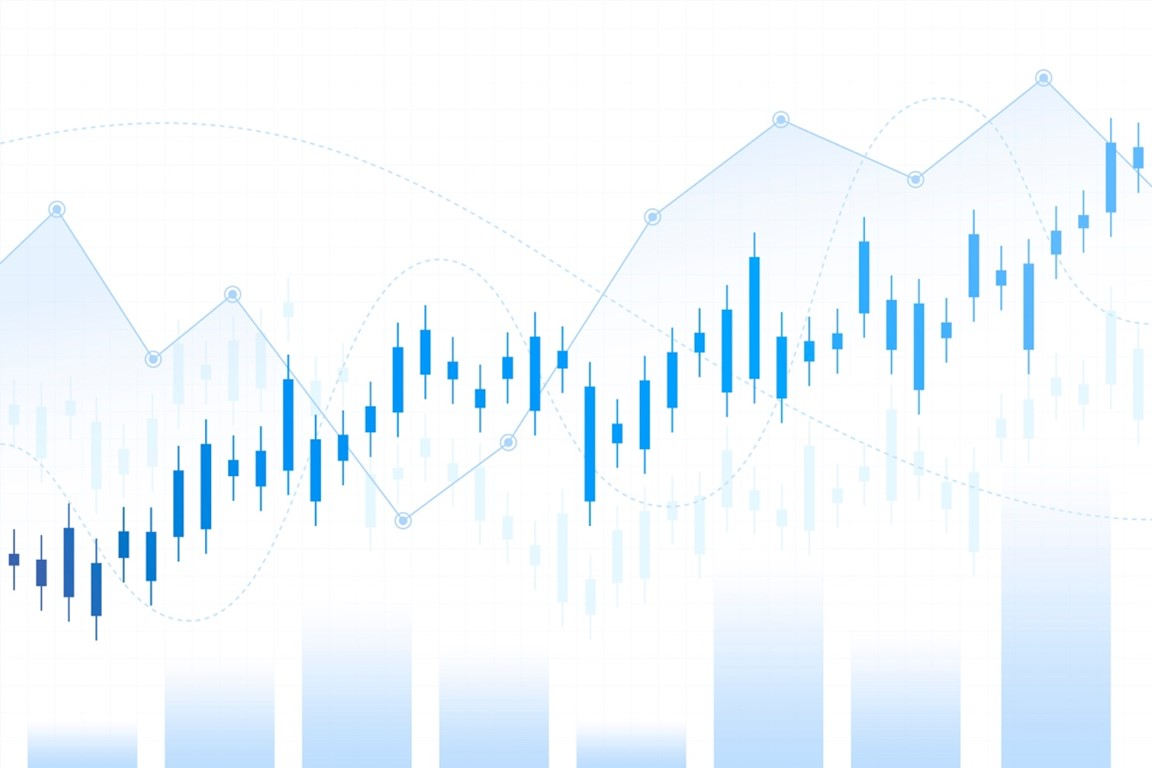
\includegraphics[width=0.6\textwidth]{Figures/Fig1.jpg} 
      \caption{This is a caption} 
      \label{fig:fig1} % Optional label for cross-referencing
    \end{figure}

\lipsum[3]

    \begin{table}[h]
      \centering
      \caption{Example Table}
      \label{tab:example}
      \begin{tabular}{ccc}
        \toprule
        \textbf{Column 1} & \textbf{Column 2} & \textbf{Column 3} \\
        \midrule
        Row 1, Col 1 & Row 1, Col 2 & Row 1, Col 3 \\
        Row 2, Col 1 & Row 2, Col 2 & Row 2, Col 3 \\
        Row 3, Col 1 & Row 3, Col 2 & Row 3, Col 3 \\
        \bottomrule
      \end{tabular}
    \end{table}

\lipsum[4]

\bibliographystyle{IEEEtran}
\bibliography{references}
\end{document}
